\lecture{1}{jeu 13 fev 2020}
\vspace{-1.2cm}

\section{Transformation Digitale}

Le monde a changé et le digital a profondément modifié nos vies, à plein de niveaux. Le marketing en est, par extension, impacté également.\\

\begin{itemize}
    \item Le "data" est partout et est devenu une des nouvelles monnaies de l'économie mondiale. Connaitre son public cible avec une grande précision, ce qui était relativement compliqué dans le passé, est devenu non seulement relativement facile, mais quasi obligatoire dans le marketing moderne.
    \item  Les consommateurs ont eux aussi changé, et leur puissance est aujourd'hui colossale: il y a environs 2.4 billions (dans le sens anglo-saxon du terme) de personnes online. Le story-telling a donc été obligé d'évoluer: avant on se focalisait sur la tâche de mettre le produit en avant, aujourd'hui la dynamique est centrée sur ce que les gens ont envie de lire ou entendre.
    \item Les news ont également changé, avec le format court et les capsules vidéos dominant le marché.
    \item La télévision a aussi profondément changé, proposant à présent des contenus multi-plateformes ou dynamiques. L'apparition de Netflix force les chaines de télévision à innover massivement, pour se démarquer. Facebook commence à également prendre beaucoup de place, avec des livestreams exclusifs d'évènements sportifs.\\
\end{itemize}

La courbe d'adoption d'un produit, à cause d'internet et du digital, a changé de forme. On est passés d'une courbe "classique" suivant une densité de probabilité de loi normale vers une courbe à la forme d'aileron de requin ("Shark fin curve"). On a donc une grande augmentation des "early adopters" et "early majority" dans les segments de marché d'Everett Rogers.

\begin{figure}[H]
\centering
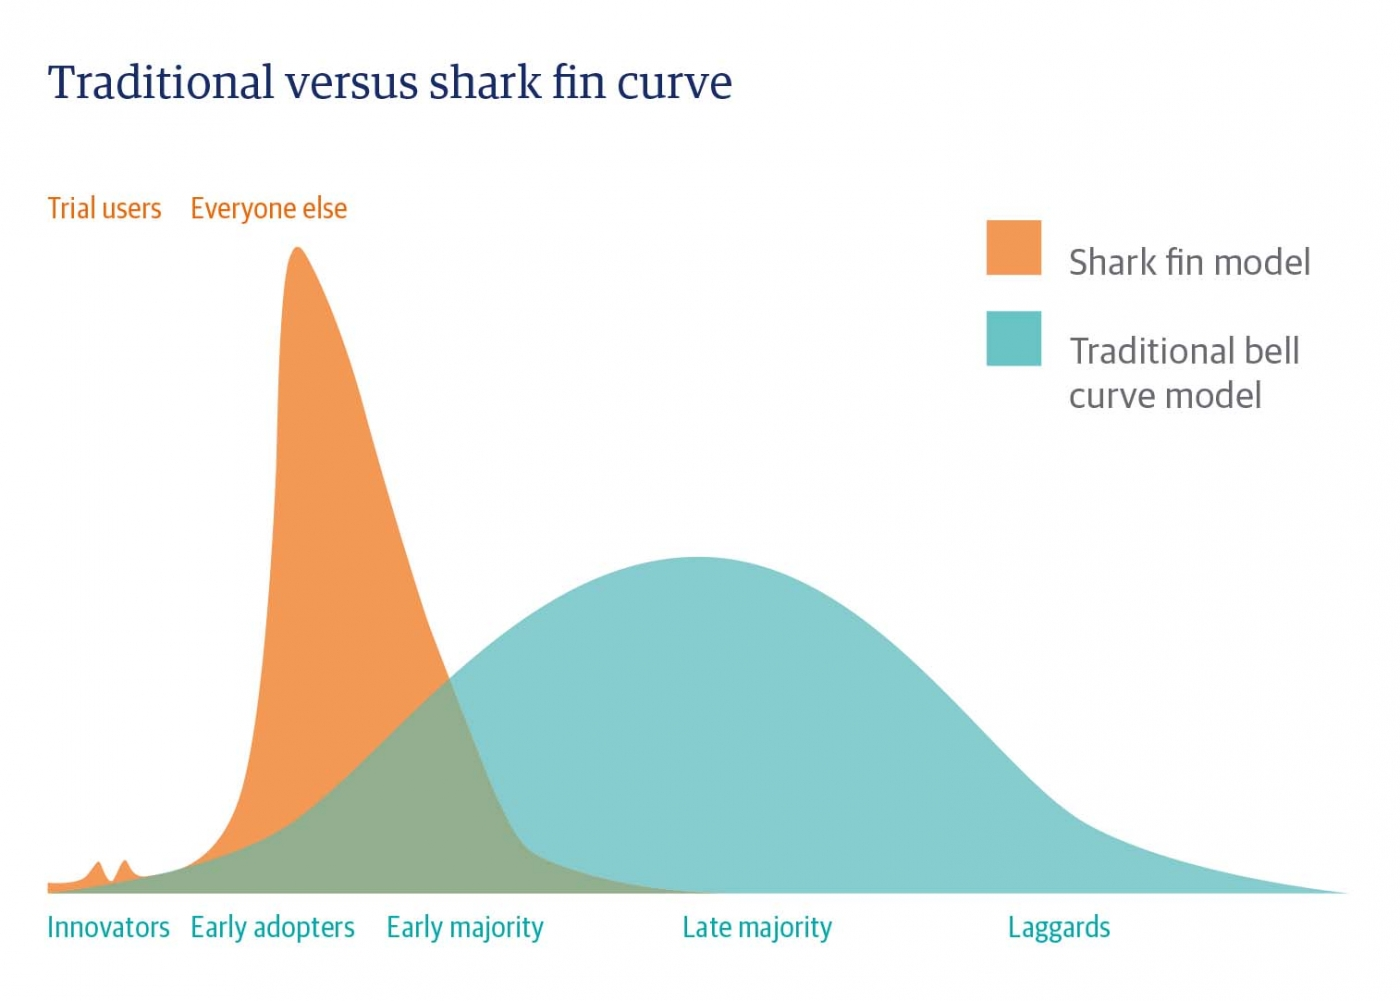
\includegraphics[scale=0.35]{../images/lec1img1}
\end{figure}

Un autre énorme changement est un shift dans le monde de la finance: les entreprises les plus riches sont maintenant des entreprises digitales (Apple, Alphabet, Microsoft, Amazon) tandis qu'avant il s'agissait d'entreprises "classiques" (dans le monde de la banque, du pétrole, pharmaceutique, etc). On voit aussi l'apparition d'entreprises au format intéressant, dont le marché principal est quelque chose qu'ils n'ont pas ou ne produisent pas: Uber ne possède pas de voitures, Alibaba ne possède pas d'inventaire personnel, Airbnb ne possède pas d'immobilier. \\

\newpage

\subsection{Les entreprises digitales et les révolutions industrielles}

Aux trois révolutions industrielles classiques qu'on a toujours connu, on ajoute aujourd'hui une quatrième, celle de la digitalisation. Klaus Schwab est le premier à avoir introduit ce concept. La technologie est maintenant intrinsèquement liée à la vie des gens, et elle permet aux nouveaux produits d'être adoptés par 100 millions d'utilisateurs très vite, ce qui prenait des années auparavant. Les demandes de brevets ont également explosé de façon exponentielle.

\begin{itemize}
    \item Première révolution industrielle: la mécanisation (machine à vapeur, machines à coudre mécanisées, l'industrie métallurgique);
    \item Deuxième révolution industrielle: l'électricité et le secteur automobile;
    \item Troisième révolution industrielle: l'invention de l'ordinateur et la découverte de l'énergie nucléaire;
    \item Quatrième révolution industrielle: la digitalisation (l'émergence de marchés nouveaux tels que les imprimantes 3D, le big data, l'intelligence artificielle, les smartphones, etc...).\\
\end{itemize}

Entre 1997 et 2006 on mettait en avant 4 entreprises comment étant celles qui avaient le plus d'influence dans le monde: les "Big Four" (Microsoft, IBM, Cisco et Intel). Depuis les années 2000 par contre, on a à deux reprises mis en avant des groupes d'entreprises à l'influence mondiale: les GAFA (Google, Apple, Facebook et Amazon) et les NATU (Netflix, Airbnb, Tesla et Uber).Le vrai impact de ces entreprises digitales est qu'elles "disruptent" toutes les industries à une vitesse folle:

\begin{itemize}
    \item Google a gagné la guerre des browsers en seulement 4 ans;
    \item Apple a vendu 3 millions de tablettes en seulement 80 jours;
    \item Facebook représente 16\% du temps de présence online des gens aux USA;
    \item Amazon a supplanté un nombre absurde de marchés en très peu d'années.
\end{itemize}

\subsection{Le business model de Google et Facebook}

Google et Facebook (tout comme d'autres entreprises, mais elles sont les plus grands exemples) ont pour source de revenus la publicité et la vente de données (ou mise à disposition, la frontière est franchement floue). Leurs core businesses: capter votre attention au plus possible et analyser vos centre d’intérêts à un degré millimétrique. En faisant cela, il leur est possible de mettre à disposition d'entreprises tierces des outils de marketing extrêmement ciblés et très pointus. \\

Facebook a comme utilisateurs, selon certaines études, 30\% de la population mondiale. L'entreprise s'implante en maître sur les réseaux sociaux, en rachetant toute concurrence directe qui grandit beaucoup trop à leur gout (par exemple Whatsapp et Instagram). Cette accumulation des données à tout prix et leurs politiques d'entreprise lui ont créé des problèmes à répétition et de nombreuses critiques:

\begin{itemize}
    \item Le scandale Cambridge Analytica;
    \item Le 10 year challenge (vu comme un simple meme au départ, il s'agissait en fait d'une façon pour Facebook pour entrainer ses algorithmes de reconnaissance faciale);
    \item La grande chute de couverture organique (Facebook était vu comme un média gratuit au départ, mais aujourd'hui la couverture organique d'un poste non-payé est d'à peine 1\%);
    \item Comme beaucoup de géants du digital, Facebook a trouvé des moyens de payer quasi rien comme impôts, tout en faisant des profits pharaoniques.\\
\end{itemize}

Suite à ça, l'évolution de la pub et la nouvelle ère de marketing est devenue celle d'influencer le bouche à oreille. Le paid media est dépassé, il faut maintenant influencer avec des messages simples, générer une grande quantité de partages et fidéliser les clients. Bien sur, des grand spécialistes qui travaillent "à l'ancienne" continuent d'exister, et ils sont très efficaces, mais ces campagnes de marketing restent extrêmement couteuses.

\subsection{Uberisation et Teslaisation}

\begin{itemize}
    \item \textbf{Uberisation} - Phénomène récent dans le domaine de l'économie consistant en l'utilisation de services permettant aux professionnels et aux clients de se mettre en contact direct, de manière quasi instantanée, grâce à l'utilisation des nouvelles technologies. La mutualisation de la gestion administrative et des infrastructures lourdes permet notamment de réduire le coût de revient de ce type de service ainsi que les poids des formalités pour les usagers. L'uberisation s'inscrit de manière plus large dans le cadre de l'économie collaborative. Exemples: Uber VS les taxis, AirBnB VS les hôtels, Blablacar et d'autres plateformes VS les transports en commun.
    \item \textbf{Teslaisation} - Tandis que l'uberisation challenge un secteur en changeant le business model existant, la teslaisation est le phénomène par lequel l'introduction d'une nouvelle technologie, initialement conçue pour une utilisation toute autre, challenge le secteur tout en gardant le même business model. Exemples: Tesla VS les fournisseurs d'énergie (leur technologie pour les batteries de voiture maintenant utilisée pour stocker de l'énergie courante, voir Powerwall), Tesla/SpaceX VS l'exploration spatiale, Tesla VS les transports publiques (voir Hyperloop), Amazon VS les autres fournisseurs de services Cloud (ouverture à tout le monde de leur technologie interne qui leur a permis de grandir).
\end{itemize}

\subsection{Exemples vus lors du cours}

\begin{itemize}
    \item \textbf{Burger King:} Campagne de Burger King pour inciter les gens à télécharger leur application mobile. "The Whopper Detour". La campagne avait pour principe d'offrir des burgers à un prix extrêmement réduit si les utilisateurs commandaient tout en étant géolocalisés à coté d'un restaurant McDonalds. Gros travail en amont pour faire du geofencing autour d'une grosse quantité de ces restaurants. L'application a été massivement téléchargée et est arrivée en numéro un des rankings sur les App Stores. Lien Youtube: \href{https://www.youtube.com/watch?v=NIWWEyPb8-Y}{THE WHOPPER DETOUR - Casefilm}
    \item \textbf{Marque italienne de boissons alcoolisées (non-nommée):} Une campagne que le professeur a lui-même géré. Avec Facebook, il est possible de geotarget un utilisateur de façon tellement fine qu'ils ont créé une campagne où ils offraient, via une pub Facebook, une boisson gratuite à des utilisateurs se trouvant physiquement dans certains restaurants italiens.
    \item \textbf{MACMA (Movimiento ayuda cáncer de mama):} Le MACMA a vu certaines de ses vidéos être retirées de Facebook. Ces vidéos étaient des tutoriels pour une autopalpation du sein afin de reconnaitre des symptômes de cancer du sein. Facebook a des règles extrêmement strictes sur la nudité féminine, mais beaucoup plus souples lorsqu'il s'agit de nudité masculine. Pour dénoncer ces standards à deux poids deux mesures, le MACMA a publié une vidéo où le tutoriel était fait sur la poitrine d'un homme, celle-ci non censurée. Lien Youtube: \href{https://www.youtube.com/watch?v=ZEbYEGrmkPg}{Movimiento Ayuda Cáncer de Mama -- Campaña "Tetas x Tetas"}
    \item \textbf{Carlings:} La marque a crée une campagne pour dénoncer l'empreinte écologique massive de la création en masse de vêtements. Avec des technologies de 3D modelling et d'OCR, ils ont crée des modèles digitaux de leurs vêtements, et via une application les utilisateurs pouvaient uploader des photos d'eux et voir ces "vêtements digitaux" s'afficher sur leurs corps. Lien Youtube: \href{https://www.youtube.com/watch?v=Sothlpxa6V0}{adDRESS THE FUTURE}
    \item \textbf{Wendy's:} Exemple d'organic advertising. Wendy's a crée un buzz multi-plateformes en utilisant le jeu Fornite. Après avoir créé un personnage dans le jeu ressemblant à leur icône, celui-ci ne s'attaquait pas aux autres joueurs, mais détruisait les frigos dans les restaurants de burgers qui se trouvaient dans le jeu (la tagline de la marque étant que leur viande n'est jamais congelée, conservant ainsi sa fraicheur). Cette attitude atypique a fait beaucoup parler les autres joueurs, qui ont ensuite fait le lien avec la marque suite à des Tweets de celle-ci (le compte de Wendy's sur Twitter est très connu aux États-Unis pour avoir une équipe de community managers extrêmement drôle et au courant des memes actuels). Suite à ça, une déferlante de streamers Twitch ont fait de la publicité gratuite à la marque. Lien Youtube: \href{https://youtu.be/DhdQmDKTBgI}{"Keeping Fortnite Fresh" - Wendy's - VMLY\&R Kansas City}
    \item \textbf{Pornhub:} Le site a des métriques de données tellement précises qu'ils étaient capables de mesurer la perte d’intérêt que les gens de la ville de Los Angeles a eu pour le match du Super Bowl en 2019, lorsque leur équipe a commencé à perdre avec une grande marge.
    \item \textbf{Netflix - Black Mirror Bandersnatch:} Netflix a proposé un nouveau type de contenu audiovisuel, permettant de choisir l'évolution du mini-film en faisant des choix à l'écran. Inspiré des livres "Choose your own adventure", ce concept avait été porté en format vidéo online pour la première fois avec des vidéos Youtube qui avaient des liens vers d'autres vidéos. Netflix n'a fait qu'adapter ce concept à un format TV.
    \item \textbf{SKAM:} Série télévisée norvégienne à grand succès, et exemple parfait des contenus multi-plateformes. Les personnages de la série avaient une présence digitale sur des plateformes telles qu'Instagram ou Facebook, et les fans pouvaient les suivre et rester en contact avec eux. Un grand nombre de capsules vidéos online étaient produits. Le concept a depuis été revendu et décliné dans un grand nombre de pays: France, Belgique, Allemagne, Italie, USA, Espagne, et Pays-Bas.
\end{itemize}
